\documentclass{beamer}
\usepackage{amsmath,amsthm,amssymb}
\usepackage{amsfonts}
\usepackage{mathtext}
\usepackage[T1,T2A]{fontenc}
\usepackage[utf8]{inputenc}
\usepackage[english,russian]{babel} 
\usepackage{mathtools}

\usepackage{latexsym}
\usepackage{import}
\usepackage{xifthen}
\usepackage{pdfpages}
\usepackage{transparent}
\usepackage{subcaption}

\newcommand{\incfig}[1]{%
    \def\svgwidth{\columnwidth}
    \import{./pictures/}{#1.pdf}
}
\pdfsuppresswarningpagegroup=1

\title{Compressed Deep Networks: Robust Low-Rank Approximation}
\author{Поздняков Григорий, Мухаметьянов Булат, Исмаилов Аким, Гарбуз Виктор, Курузов Илья}

\begin{document}% начало презентации

\begin{frame}% первый слайд
\titlepage
\end{frame}

\begin{frame}
Для примера выполним приближение для матрицы 
$\begin{pmatrix}
  3 & 5\\
  0 & 1
 \end{pmatrix}
$
\end{frame}

\begin{frame}
$\|Av_{max}\| = 4.205048581$  
    \begin{figure}
    \begin{subfigure}{.5\textwidth}
        \centering
        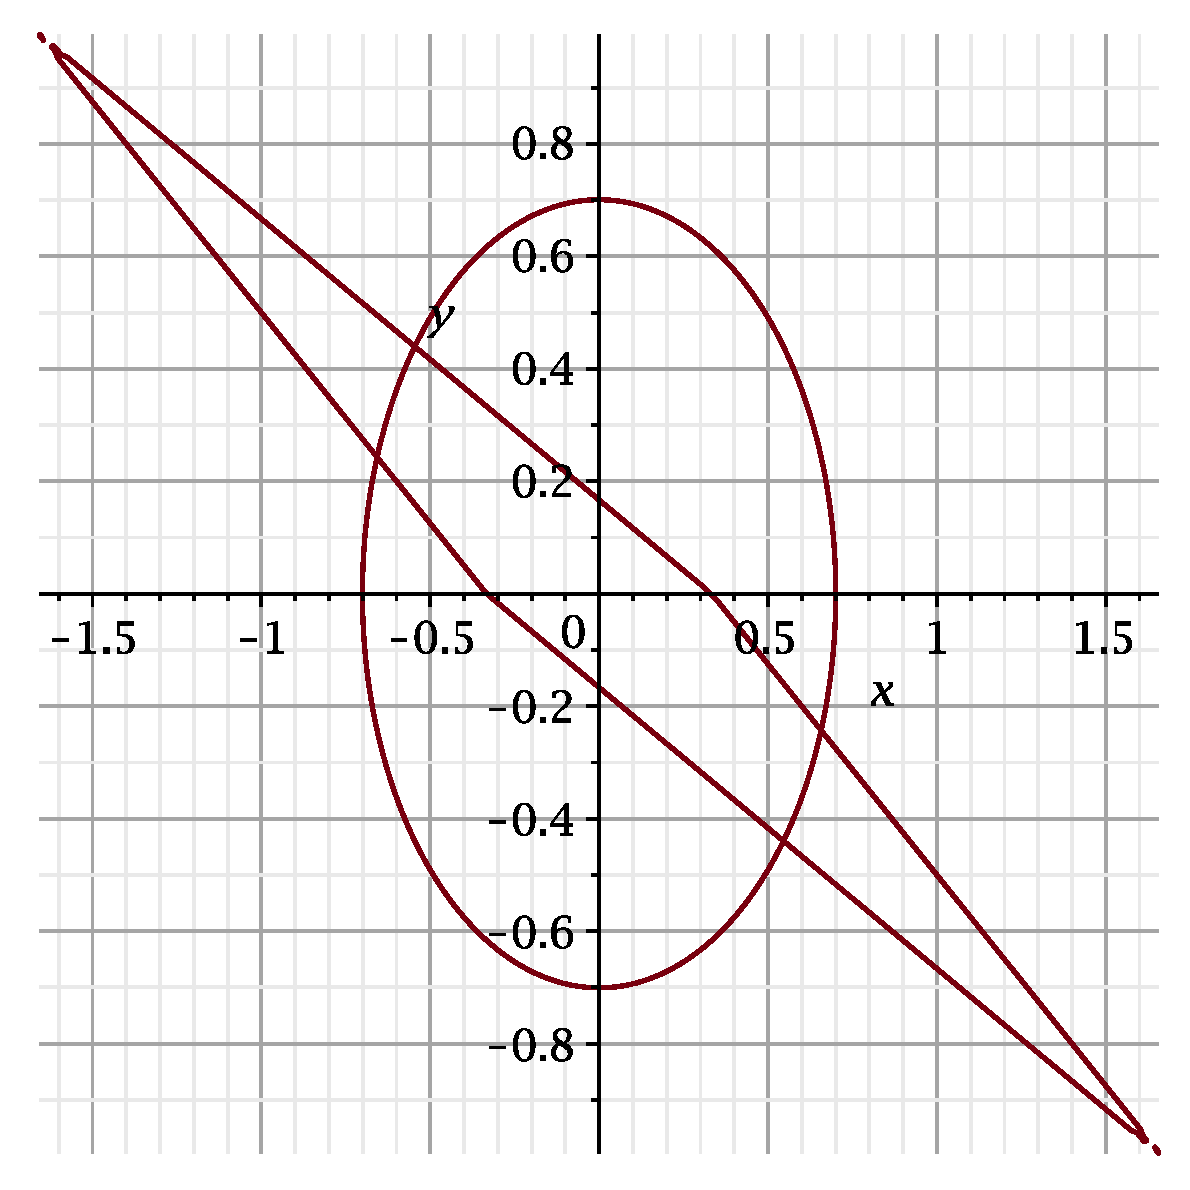
\includegraphics[width=.8\linewidth]{pictures/1.eps}
        \caption{$\displaystyle\frac{1}{d}(E-c)+c$}
    \label{fig:sfig1}
    \end{subfigure}%
    \begin{subfigure}{.5\textwidth}
        \centering
        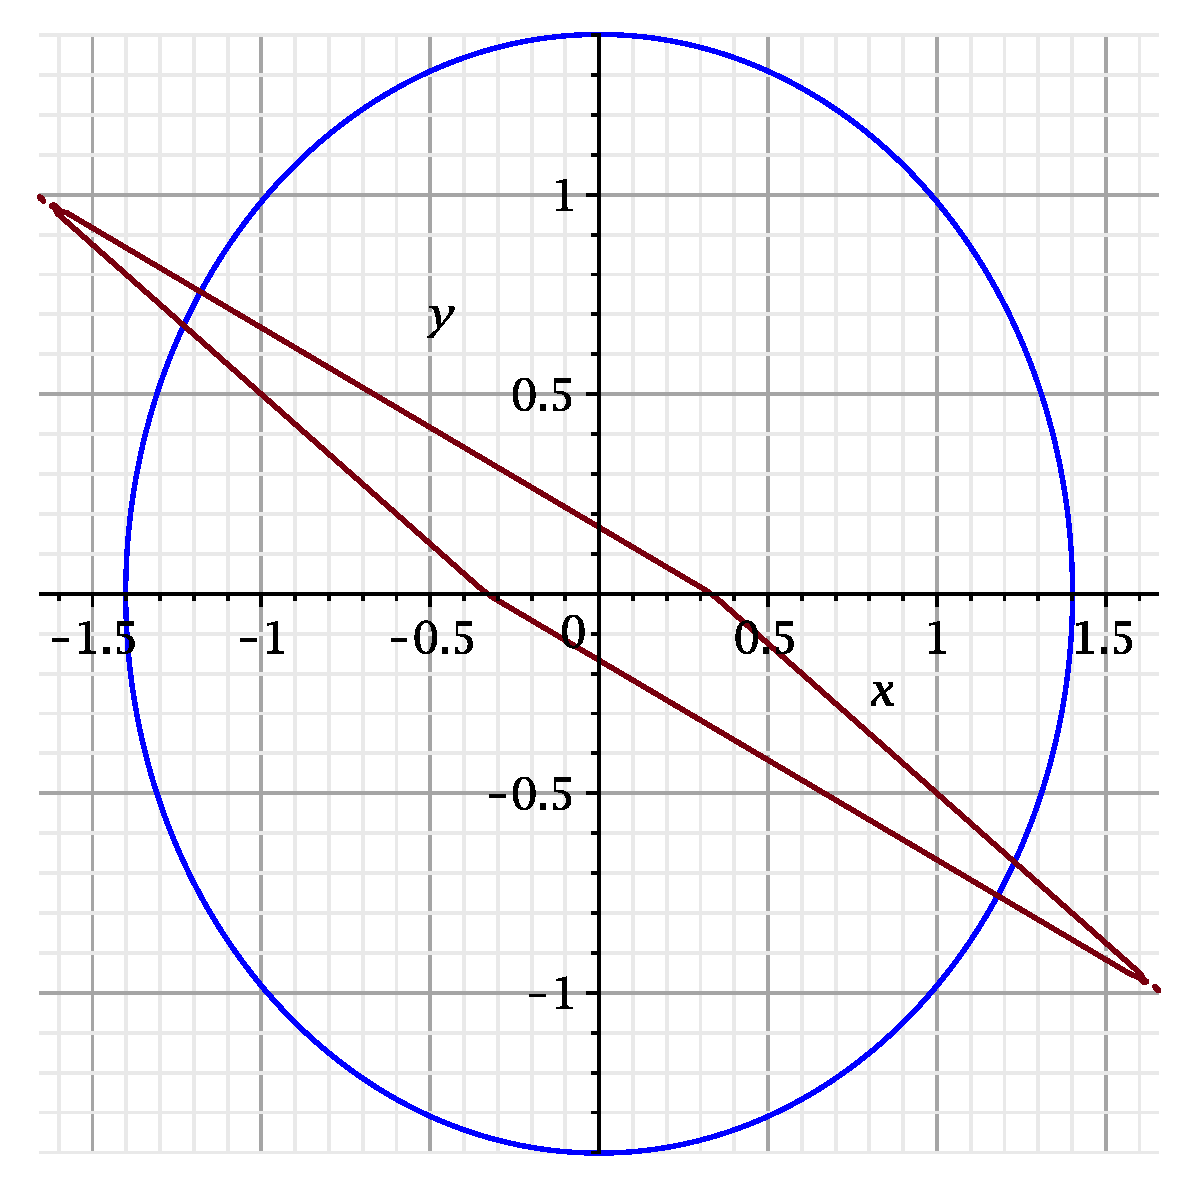
\includegraphics[width=.8\linewidth]{pictures/1_1.eps}
        \caption{E}
    \label{fig:sfig2}
    \end{subfigure}
\end{figure}

\end{frame}

\begin{frame}
$\|Av_{max}\| = 1.870191875$  
    \begin{figure}
    \begin{subfigure}{.5\textwidth}
        \centering
        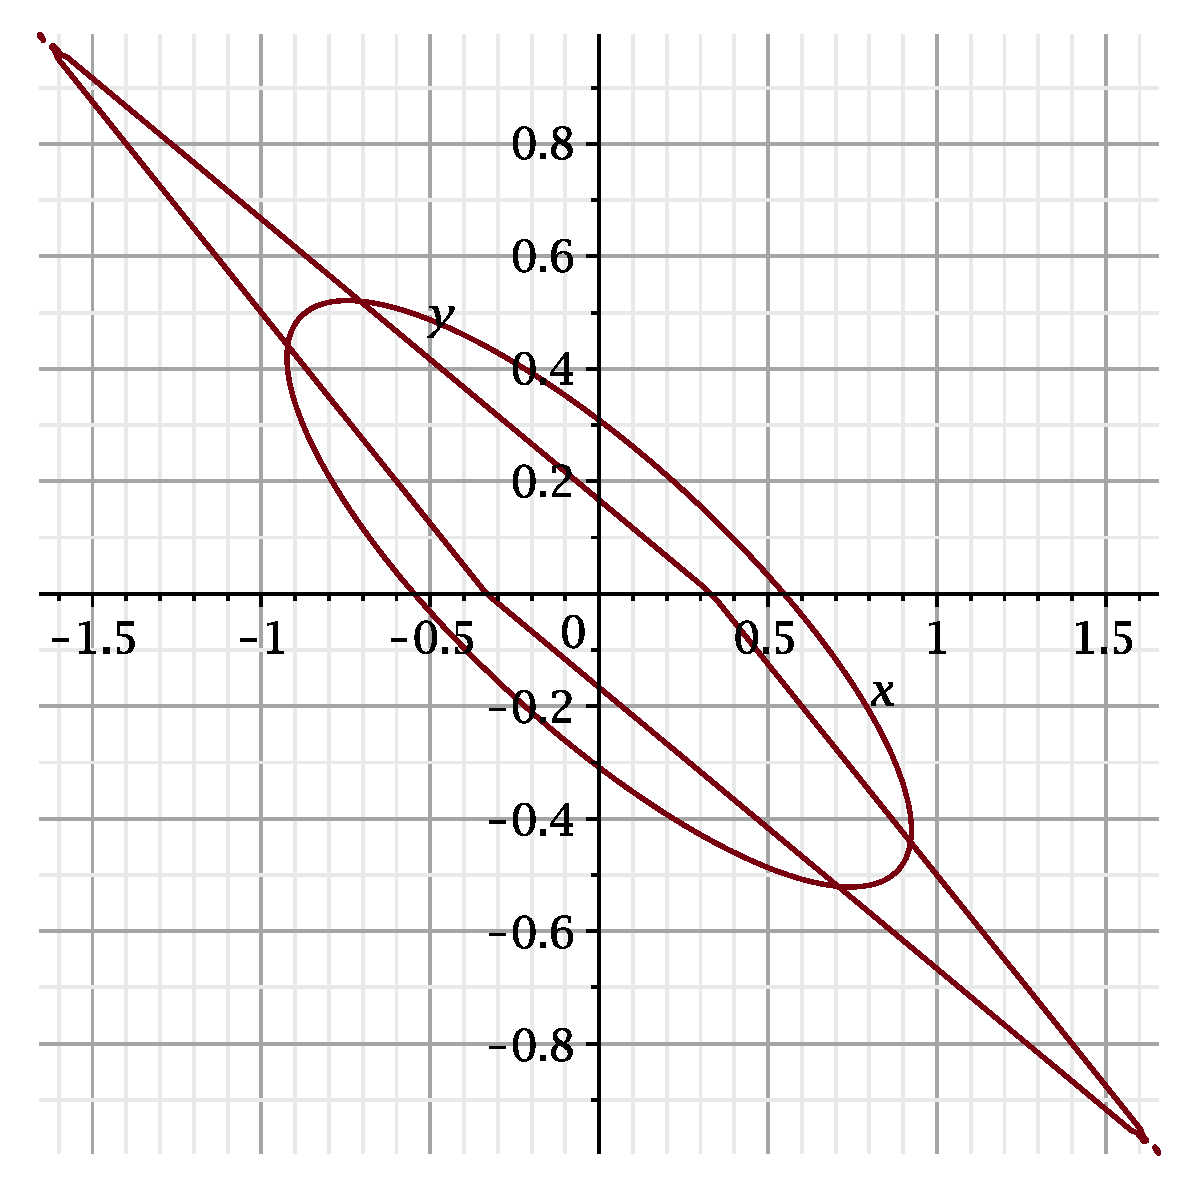
\includegraphics[width=.8\linewidth]{pictures/2.eps}
        \caption{$\displaystyle\frac{1}{d}(E-c)+c$}
    \label{fig:sfig1}
    \end{subfigure}%
    \begin{subfigure}{.5\textwidth}
        \centering
        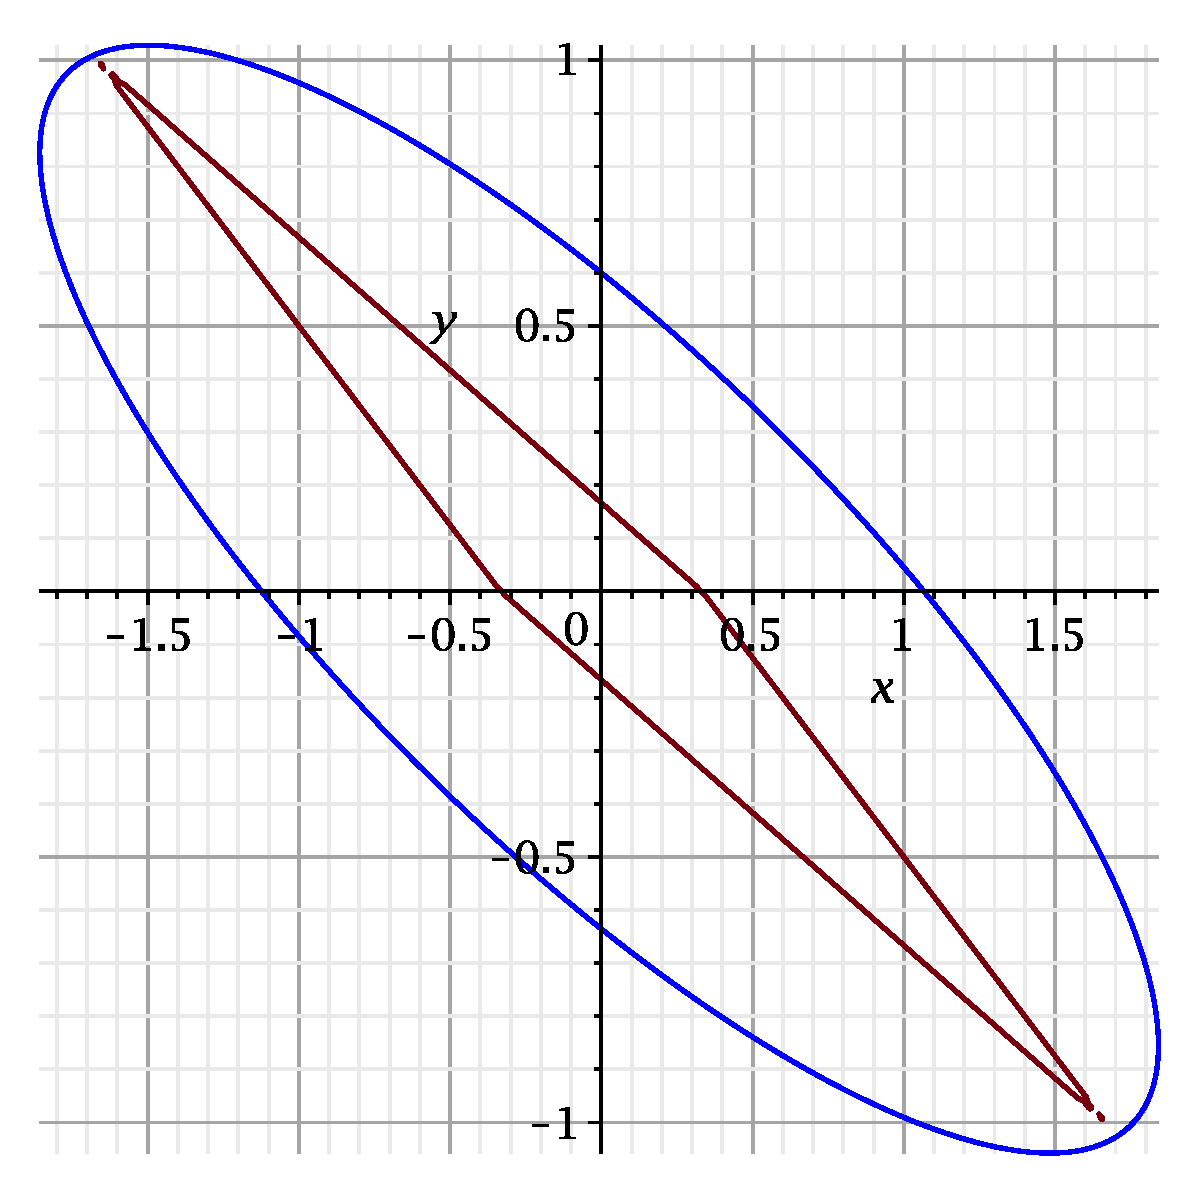
\includegraphics[width=.8\linewidth]{pictures/1_2.eps}
        \caption{E}
    \label{fig:sfig2}
    \end{subfigure}
\end{figure}

\end{frame}

\begin{frame}
$\|Av_{max}\| = 1.673897363$  
    \begin{figure}
    \begin{subfigure}{.5\textwidth}
        \centering
        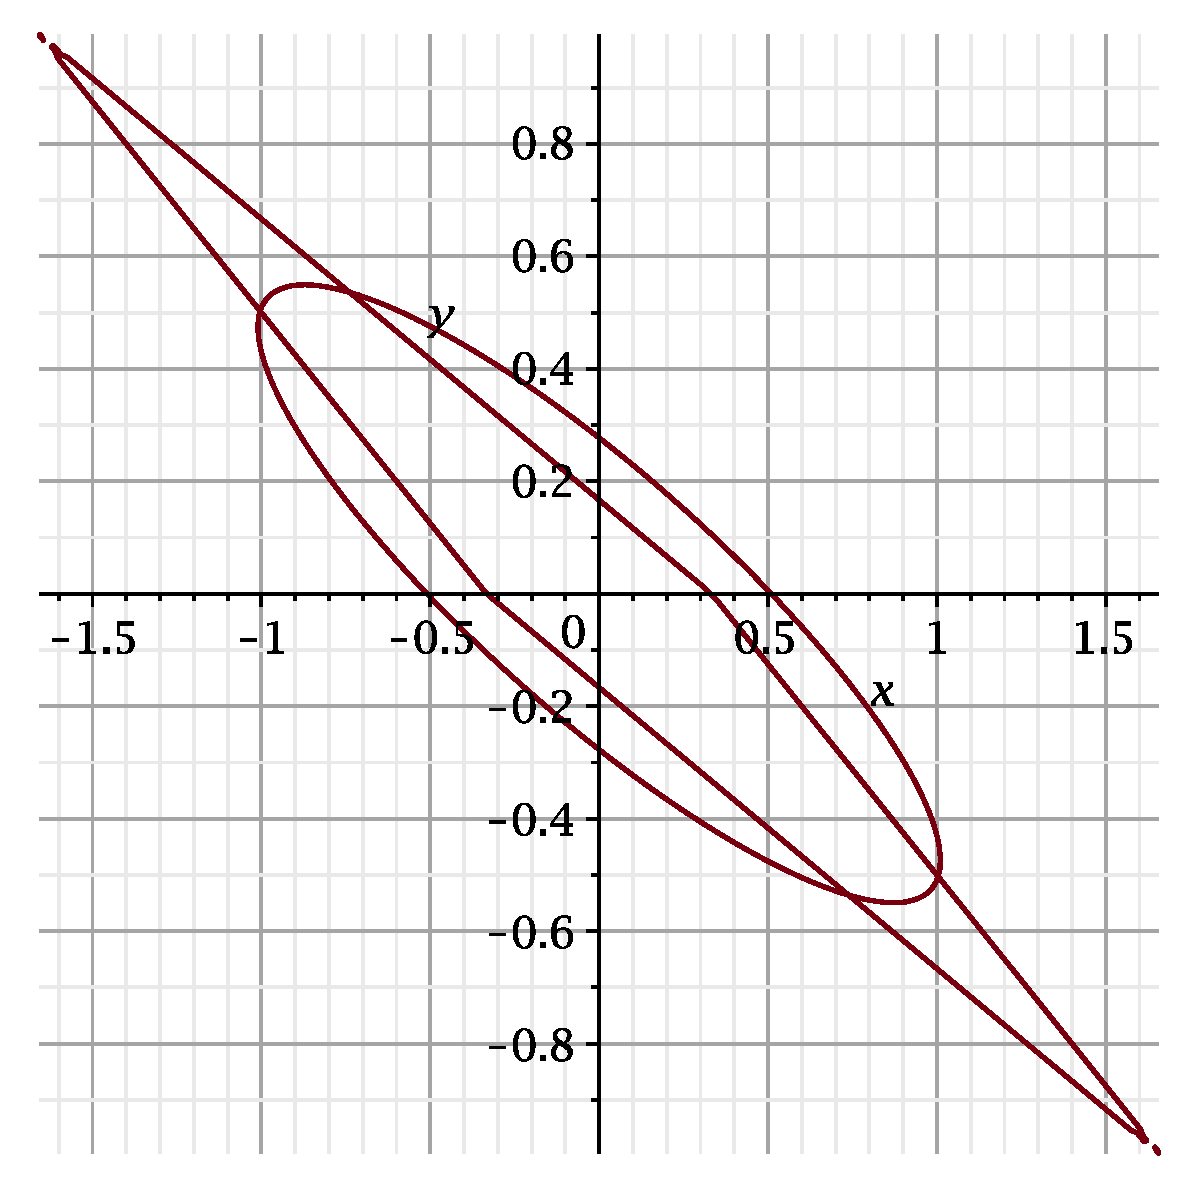
\includegraphics[width=.8\linewidth]{pictures/3.eps}
        \caption{$\displaystyle\frac{1}{d}(E-c)+c$}
    \label{fig:sfig1}
    \end{subfigure}%
    \begin{subfigure}{.5\textwidth}
        \centering
        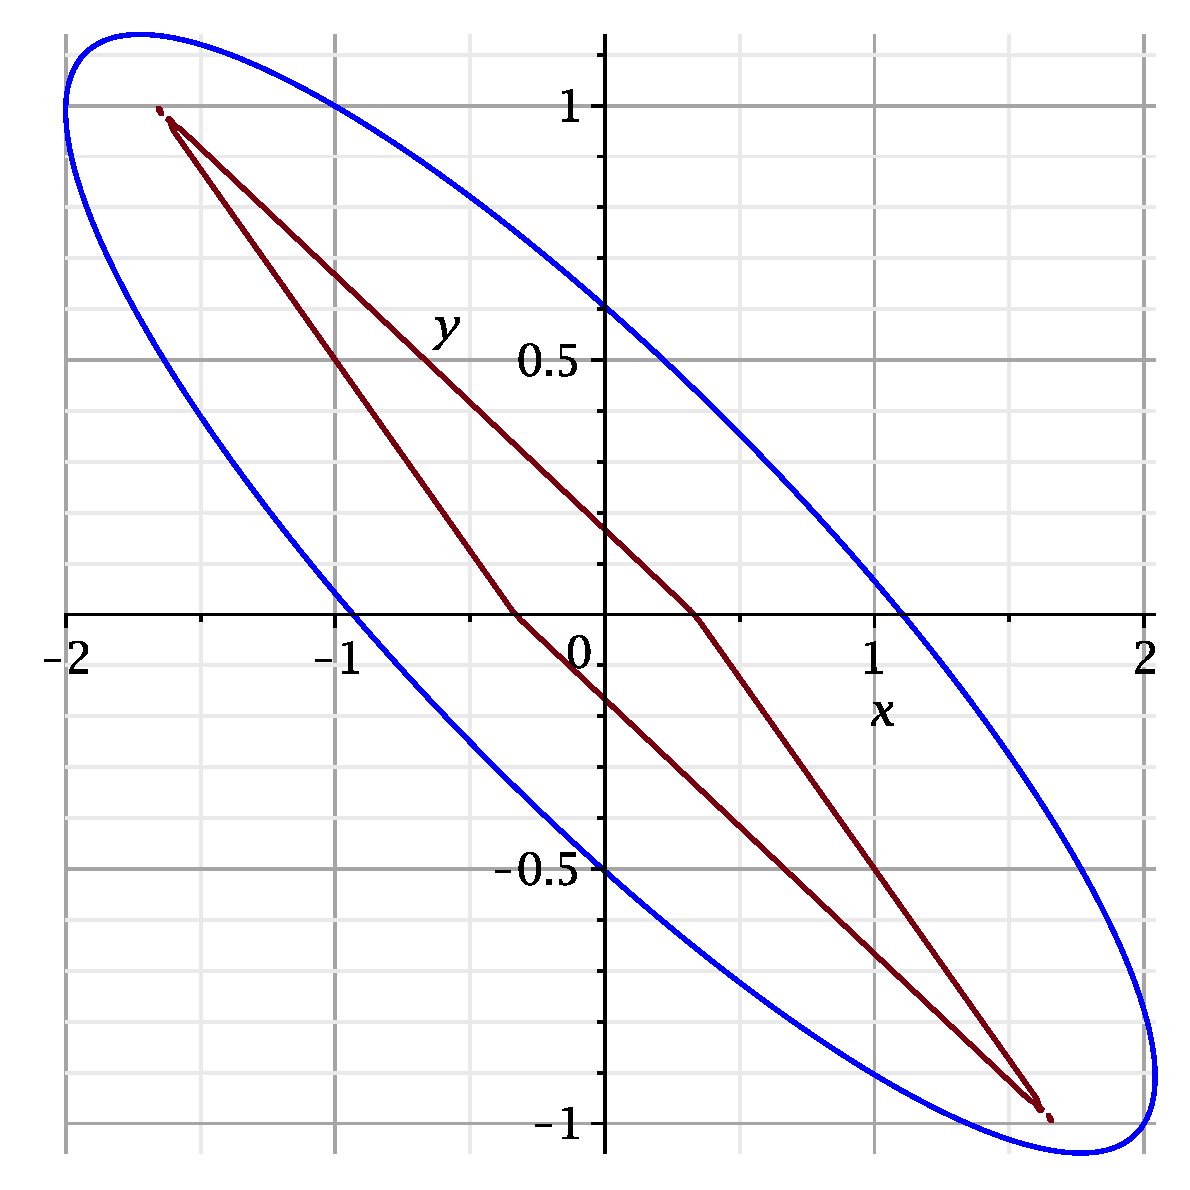
\includegraphics[width=.8\linewidth]{pictures/1_3.eps}
        \caption{E}
    \label{fig:sfig2}
    \end{subfigure}
\end{figure}

\end{frame}

\begin{frame}
$\|Av_{max}\| = 1.498205836$  
    \begin{figure}
    \begin{subfigure}{.5\textwidth}
        \centering
        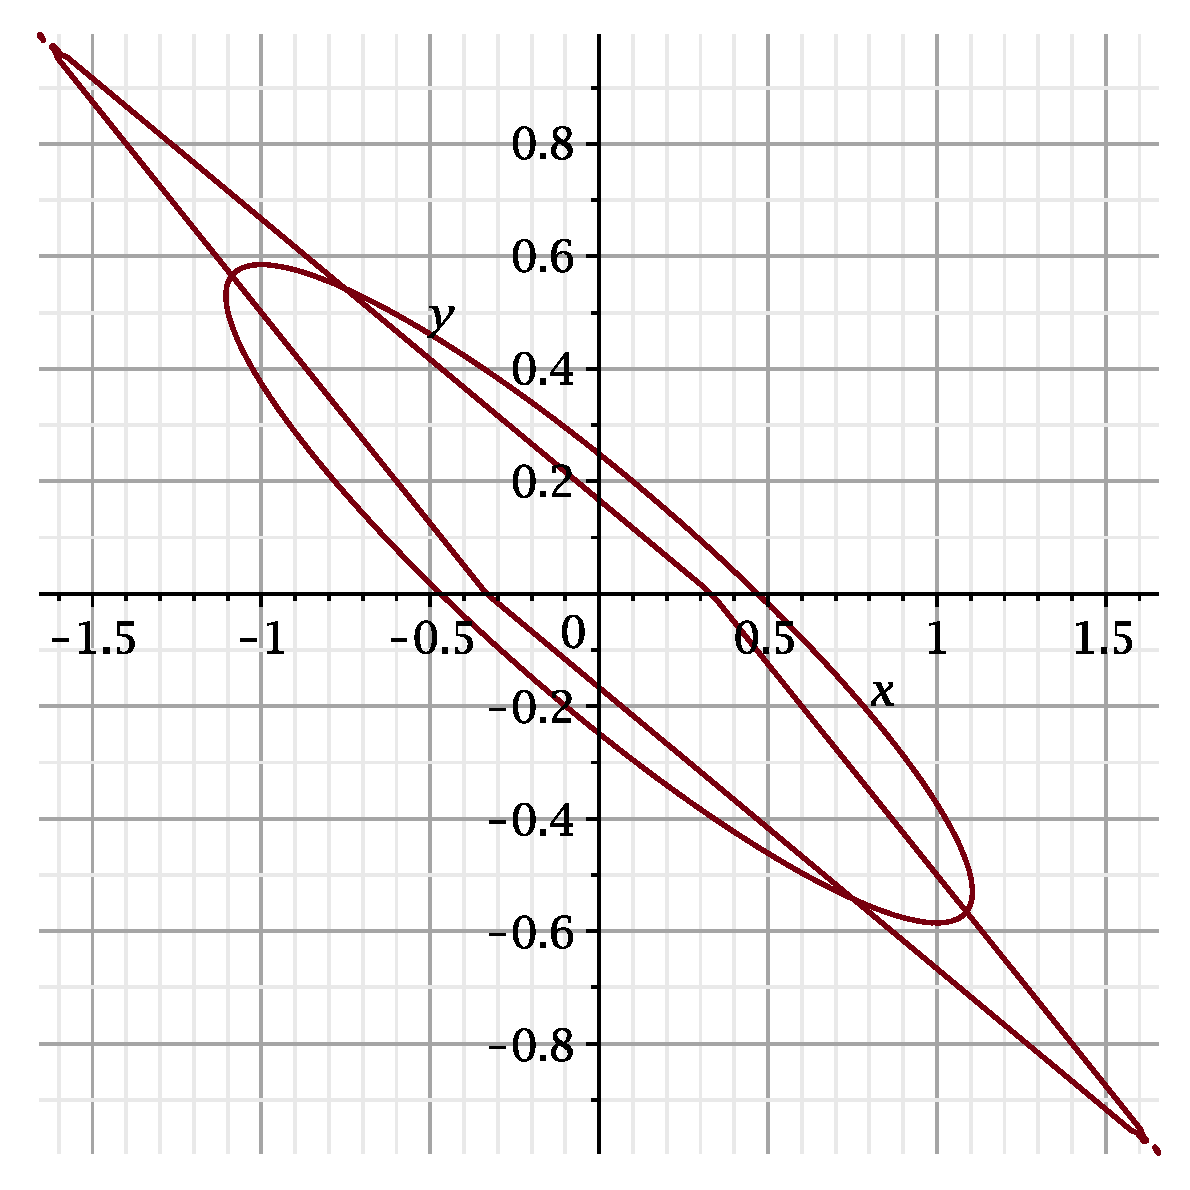
\includegraphics[width=.8\linewidth]{pictures/4.eps}
        \caption{$\displaystyle\frac{1}{d}(E-c)+c$}
    \label{fig:sfig1}
    \end{subfigure}%
    \begin{subfigure}{.5\textwidth}
        \centering
        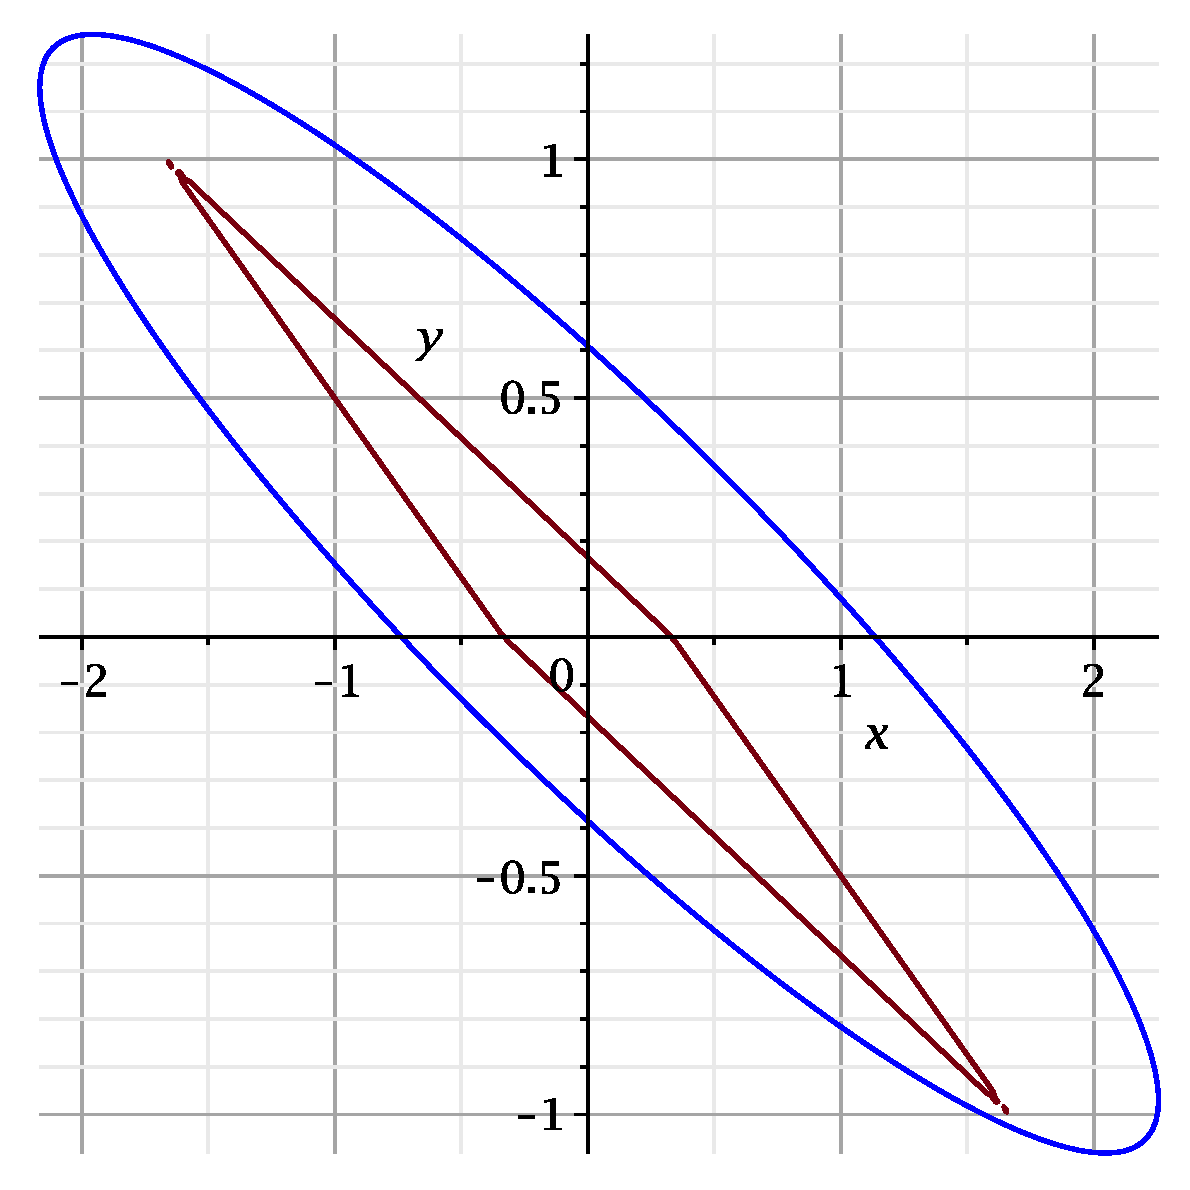
\includegraphics[width=.8\linewidth]{pictures/1_4.eps}
        \caption{E}
    \label{fig:sfig2}
    \end{subfigure}
\end{figure}

\end{frame}

\begin{frame}
$\|Av_{max}\| = 1.393561122$  
    \begin{figure}
    \begin{subfigure}{.5\textwidth}
        \centering
        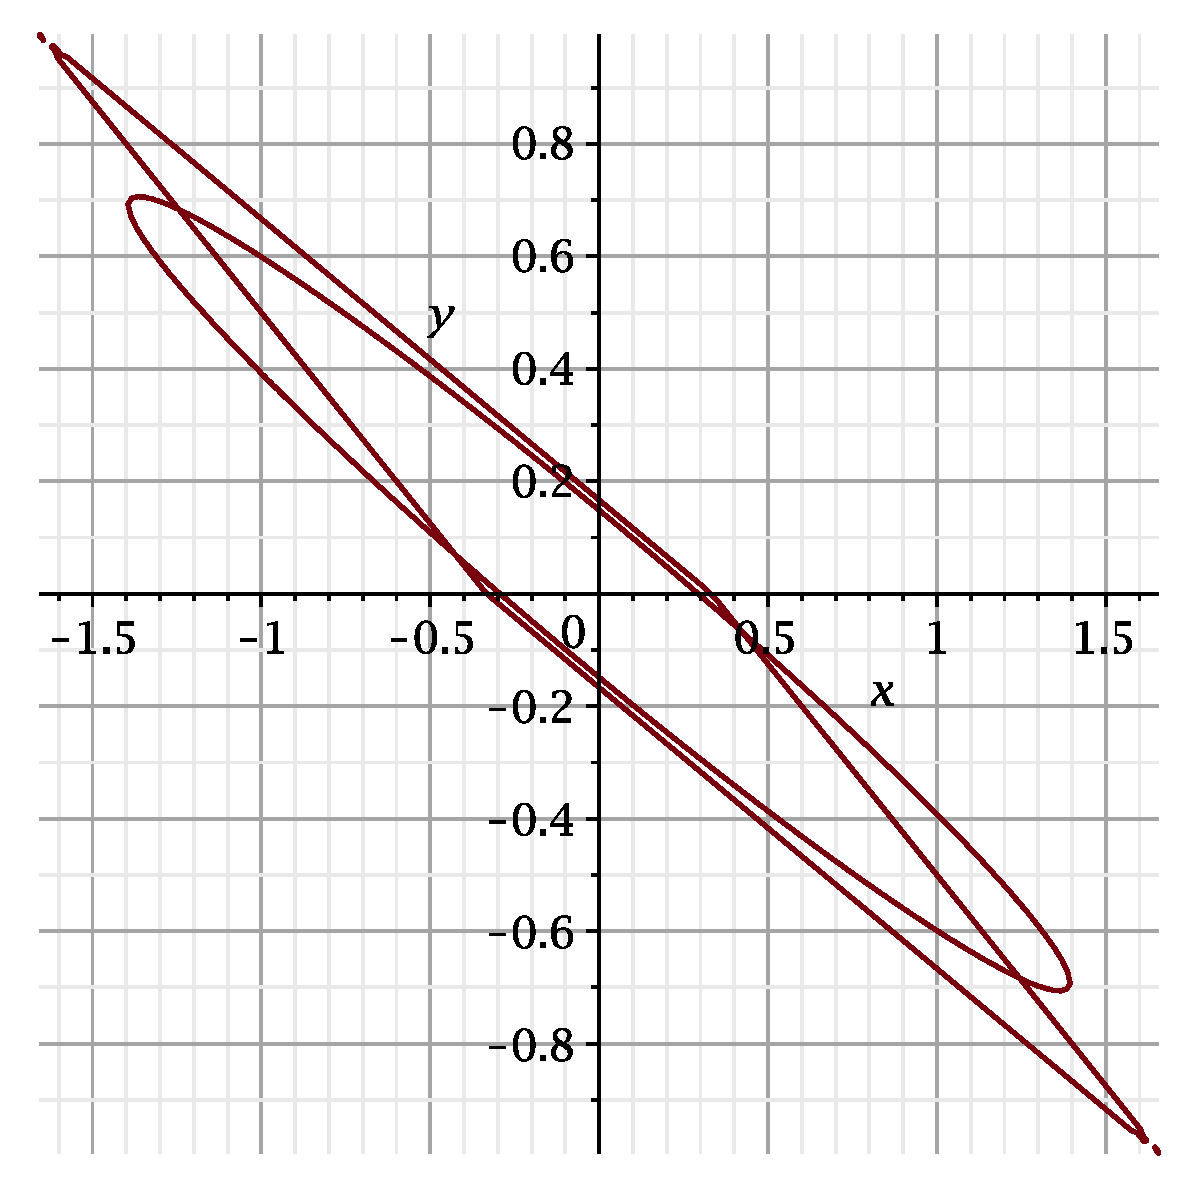
\includegraphics[width=.8\linewidth]{pictures/5.eps}
        \caption{$\displaystyle\frac{1}{d}(E-c)+c$}
    \label{fig:sfig1}
    \end{subfigure}%
    \begin{subfigure}{.5\textwidth}
        \centering
        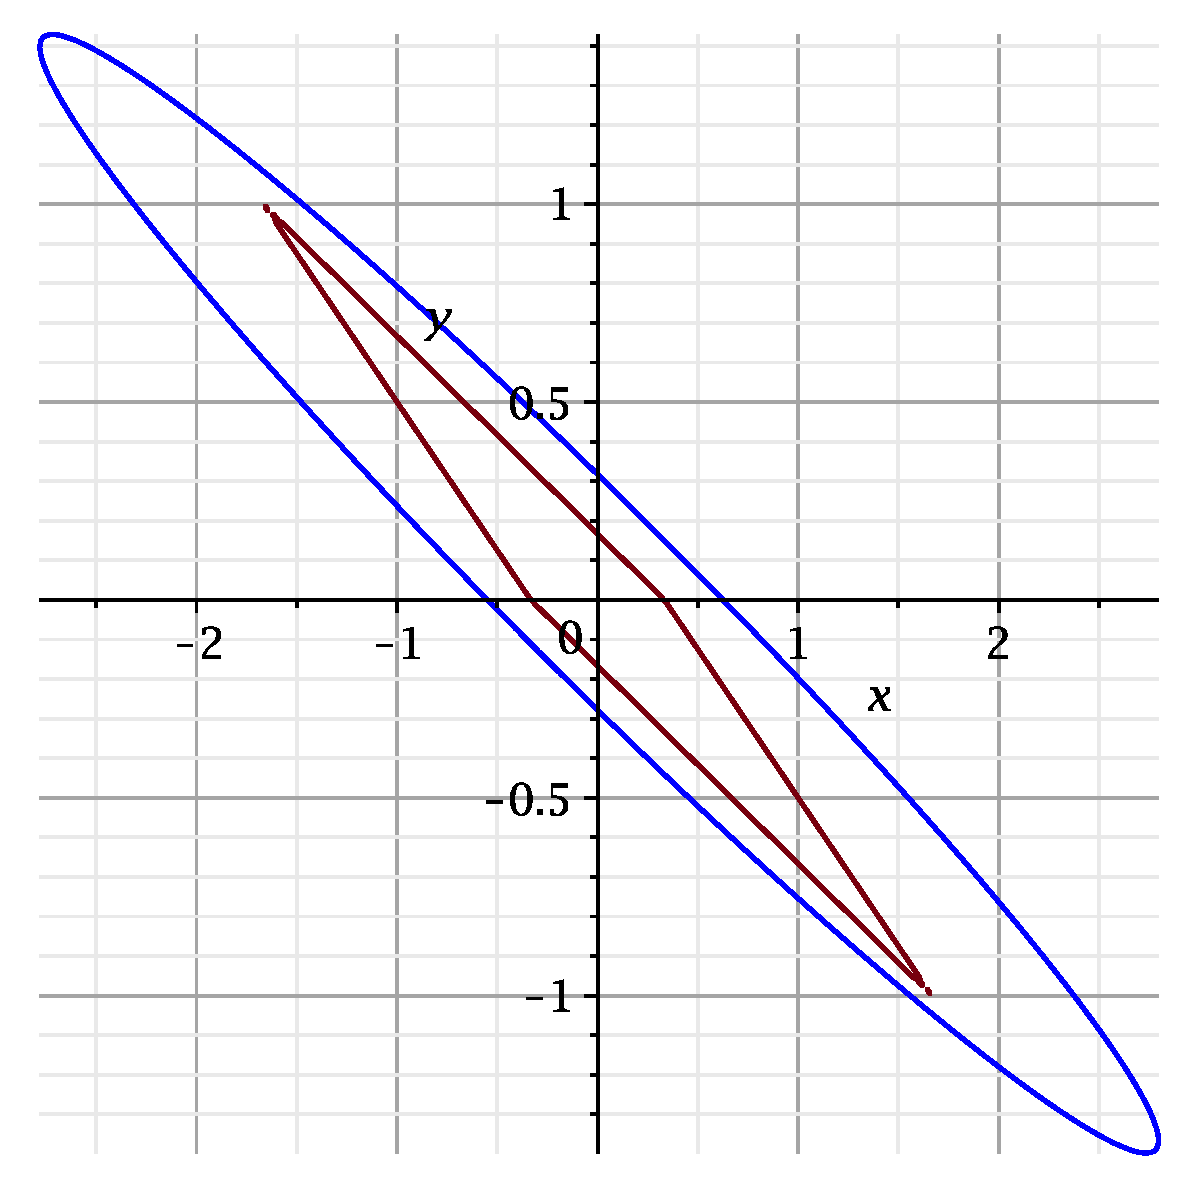
\includegraphics[width=.8\linewidth]{pictures/1_5.eps}
        \caption{E}
    \label{fig:sfig2}
    \end{subfigure}
\end{figure}

\end{frame}

\begin{frame}
$\|Av_{max}\| = 1.193351619$  
    \begin{figure}
    \begin{subfigure}{.5\textwidth}
        \centering
        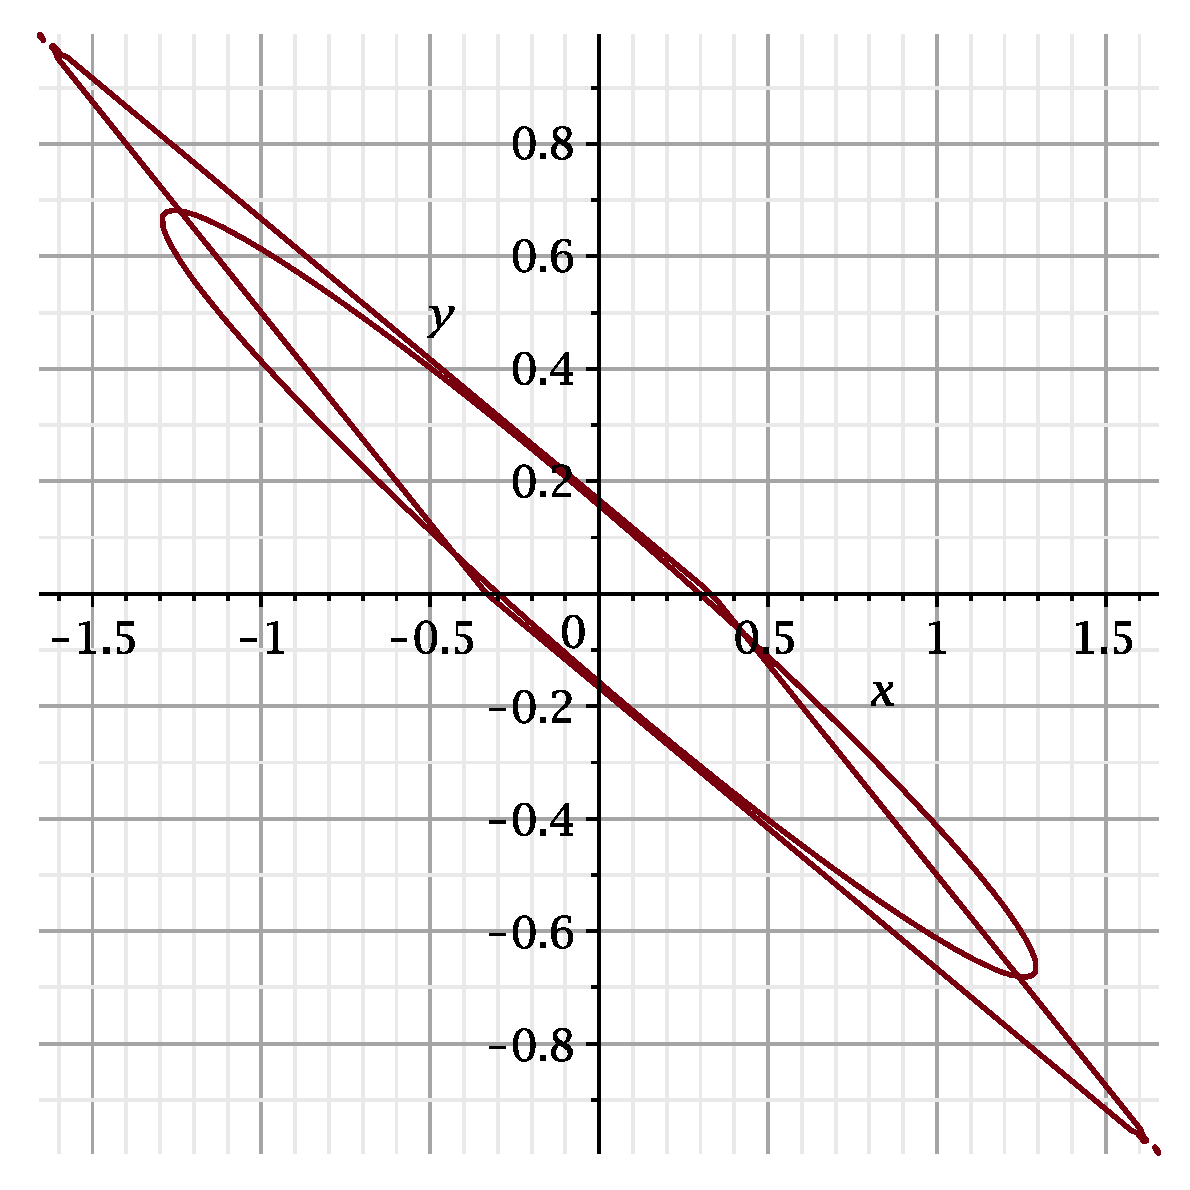
\includegraphics[width=.8\linewidth]{pictures/6.eps}
        \caption{$\displaystyle\frac{1}{d}(E-c)+c$}
    \label{fig:sfig1}
    \end{subfigure}%
    \begin{subfigure}{.5\textwidth}
        \centering
        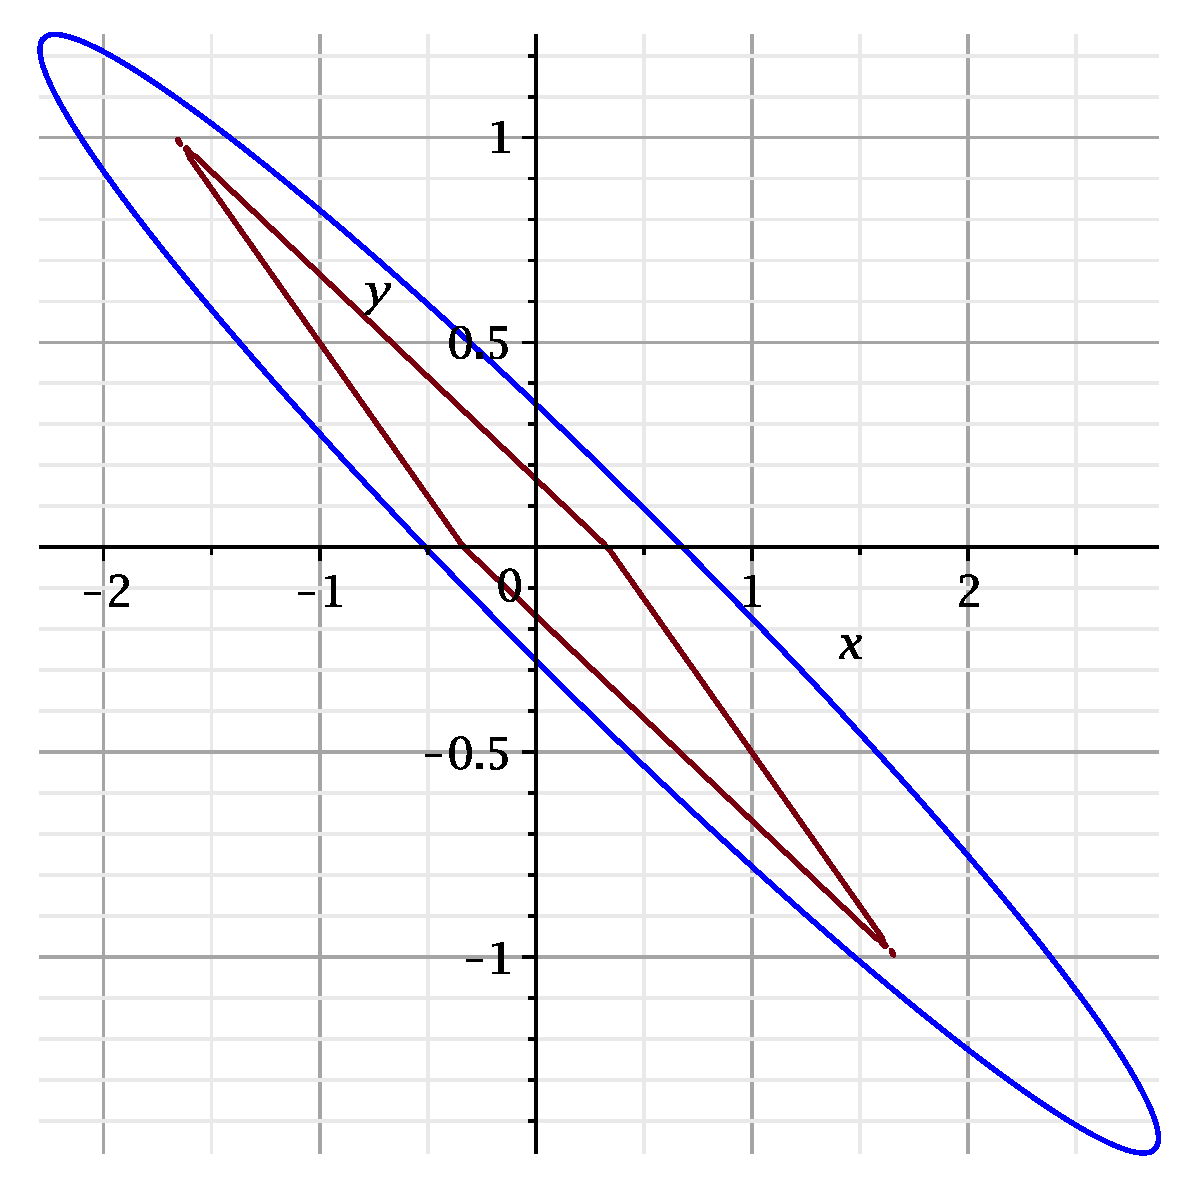
\includegraphics[width=.8\linewidth]{pictures/1_6.eps}
        \caption{E}
    \label{fig:sfig2}
    \end{subfigure}
\end{figure}

\end{frame}

\begin{frame}
$\|Av_{max}\| = 1.005507172$  
    \begin{figure}
    \begin{subfigure}{.5\textwidth}
        \centering
        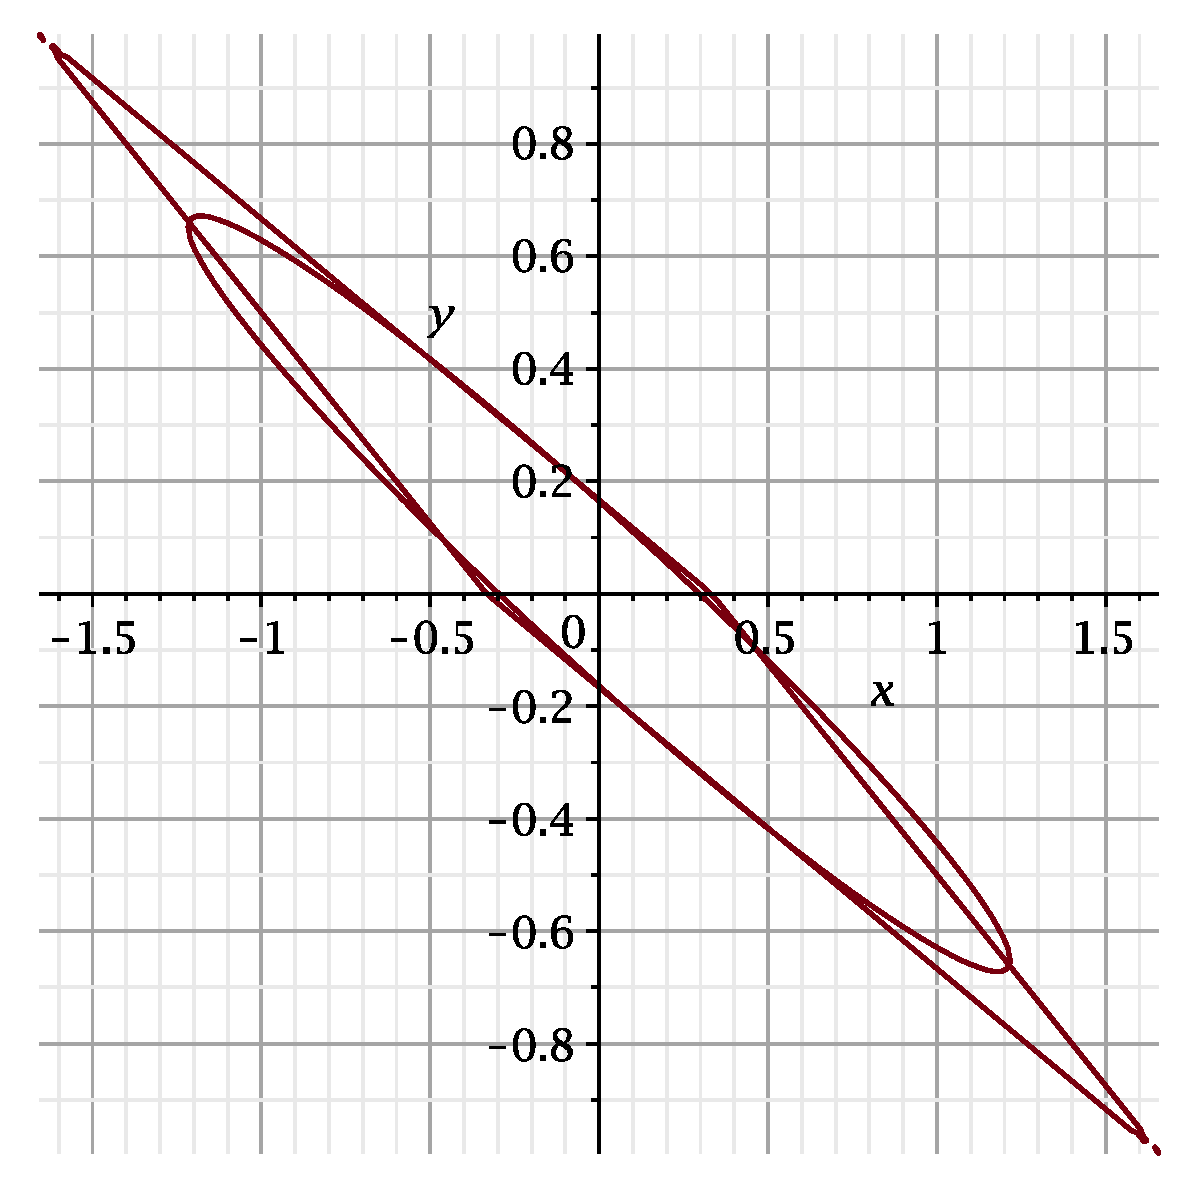
\includegraphics[width=.8\linewidth]{pictures/7.eps}
        \caption{$\displaystyle\frac{1}{d}(E-c)+c$}
    \label{fig:sfig1}
    \end{subfigure}%
    \begin{subfigure}{.5\textwidth}
        \centering
        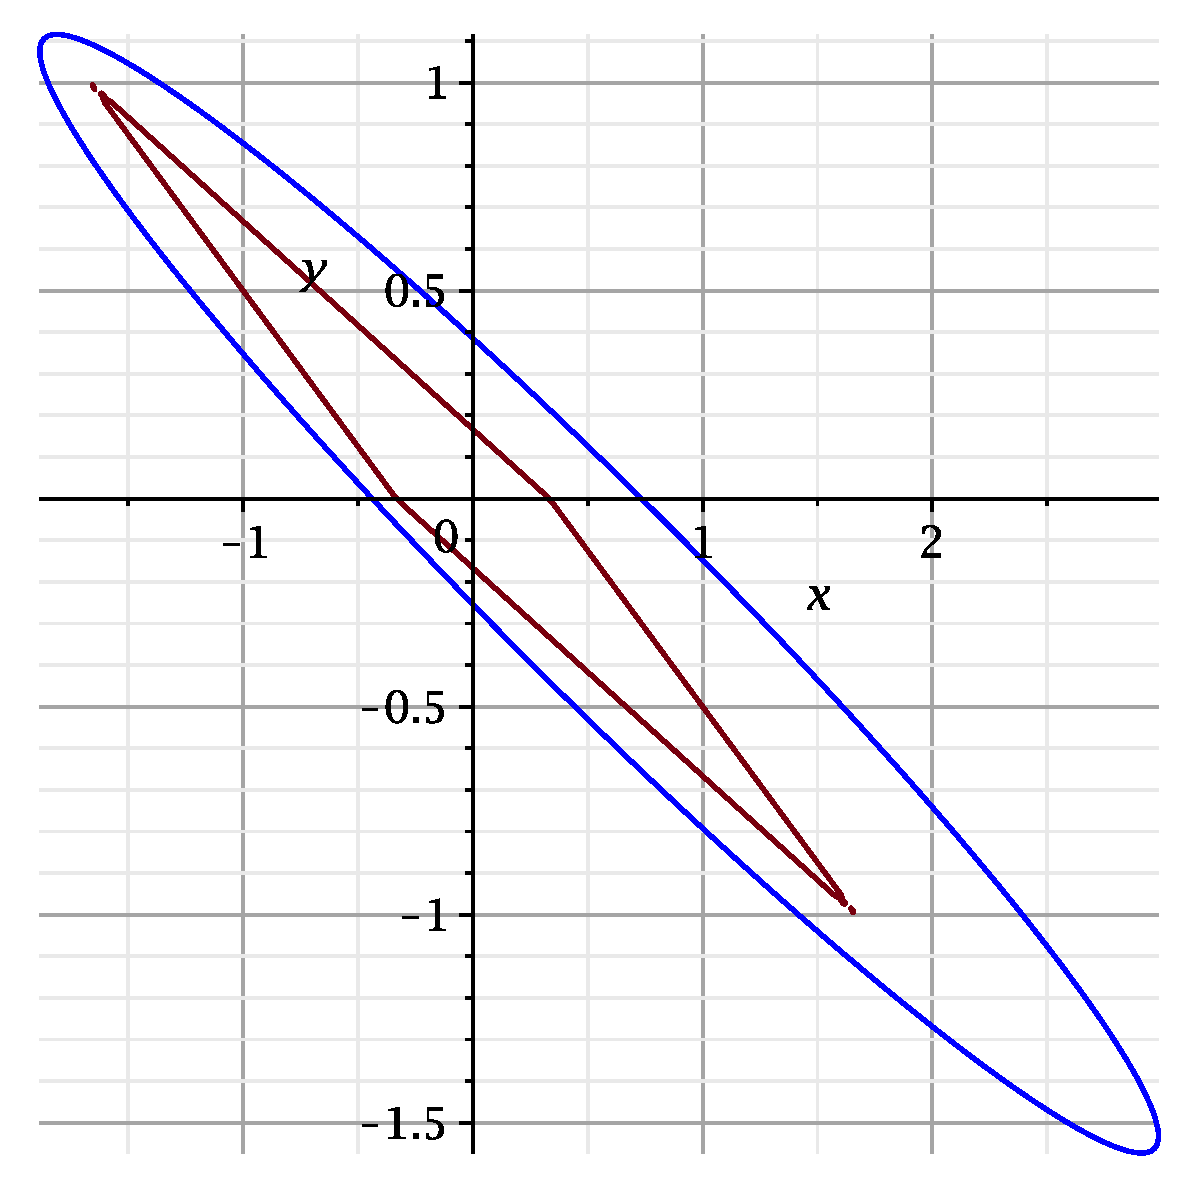
\includegraphics[width=.8\linewidth]{pictures/1_7.eps}
        \caption{E}
    \label{fig:sfig2}
    \end{subfigure}
\end{figure}

\end{frame}

\begin{frame}
$\|Av_{max}\| = 0.9316673493$  
    \begin{figure}
    \begin{subfigure}{.5\textwidth}
        \centering
        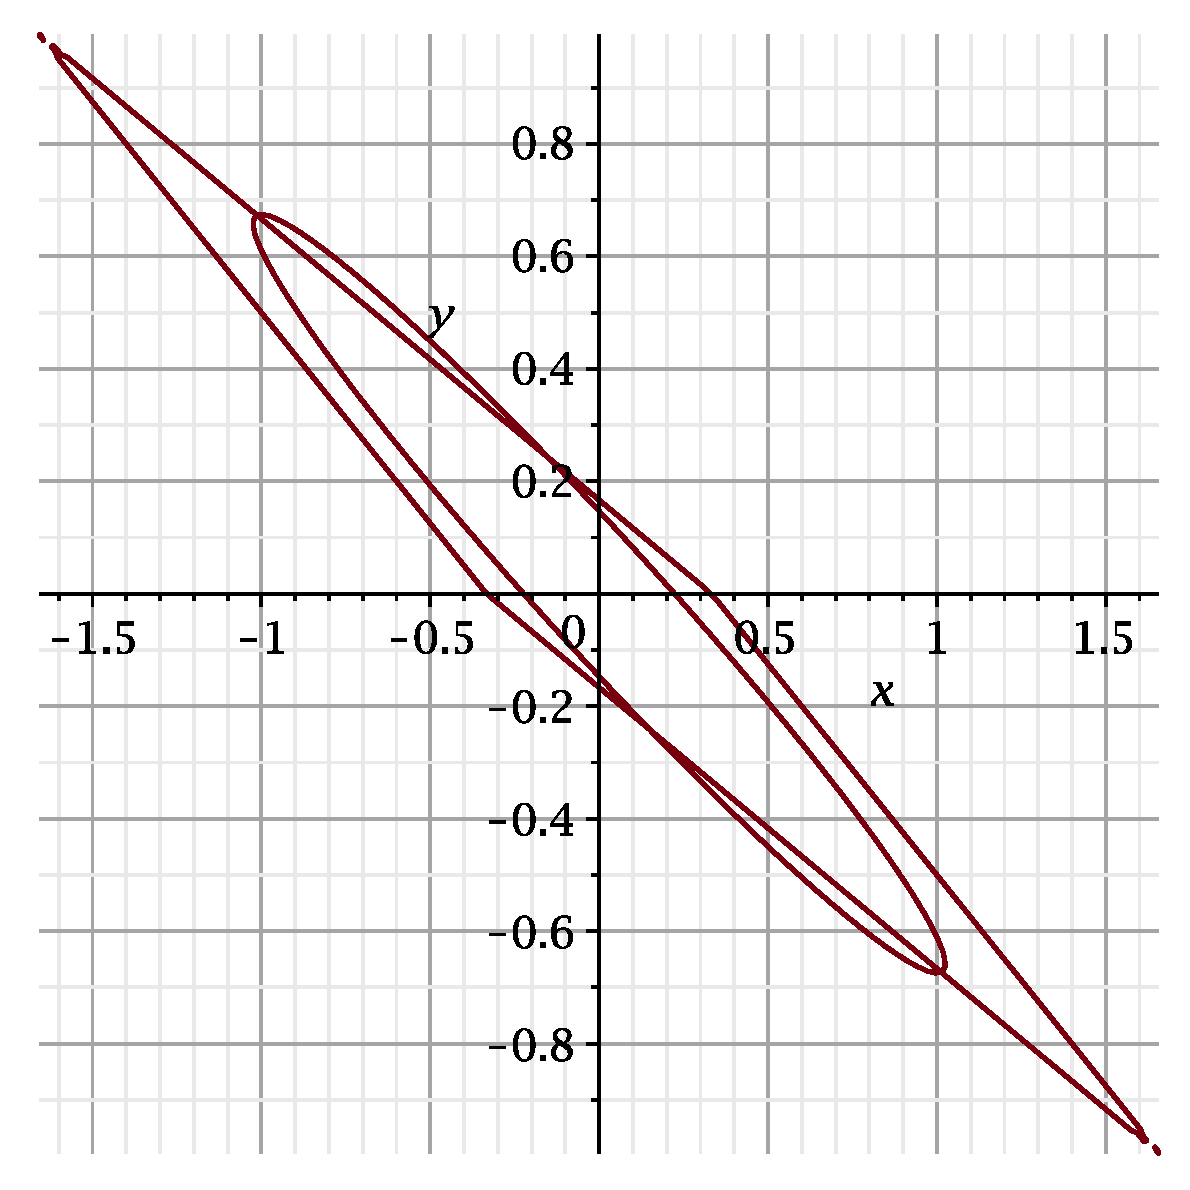
\includegraphics[width=.8\linewidth]{pictures/8.eps}
        \caption{$\displaystyle\frac{1}{d}(E-c)+c$}
    \label{fig:sfig1}
    \end{subfigure}%
    \begin{subfigure}{.5\textwidth}
        \centering
        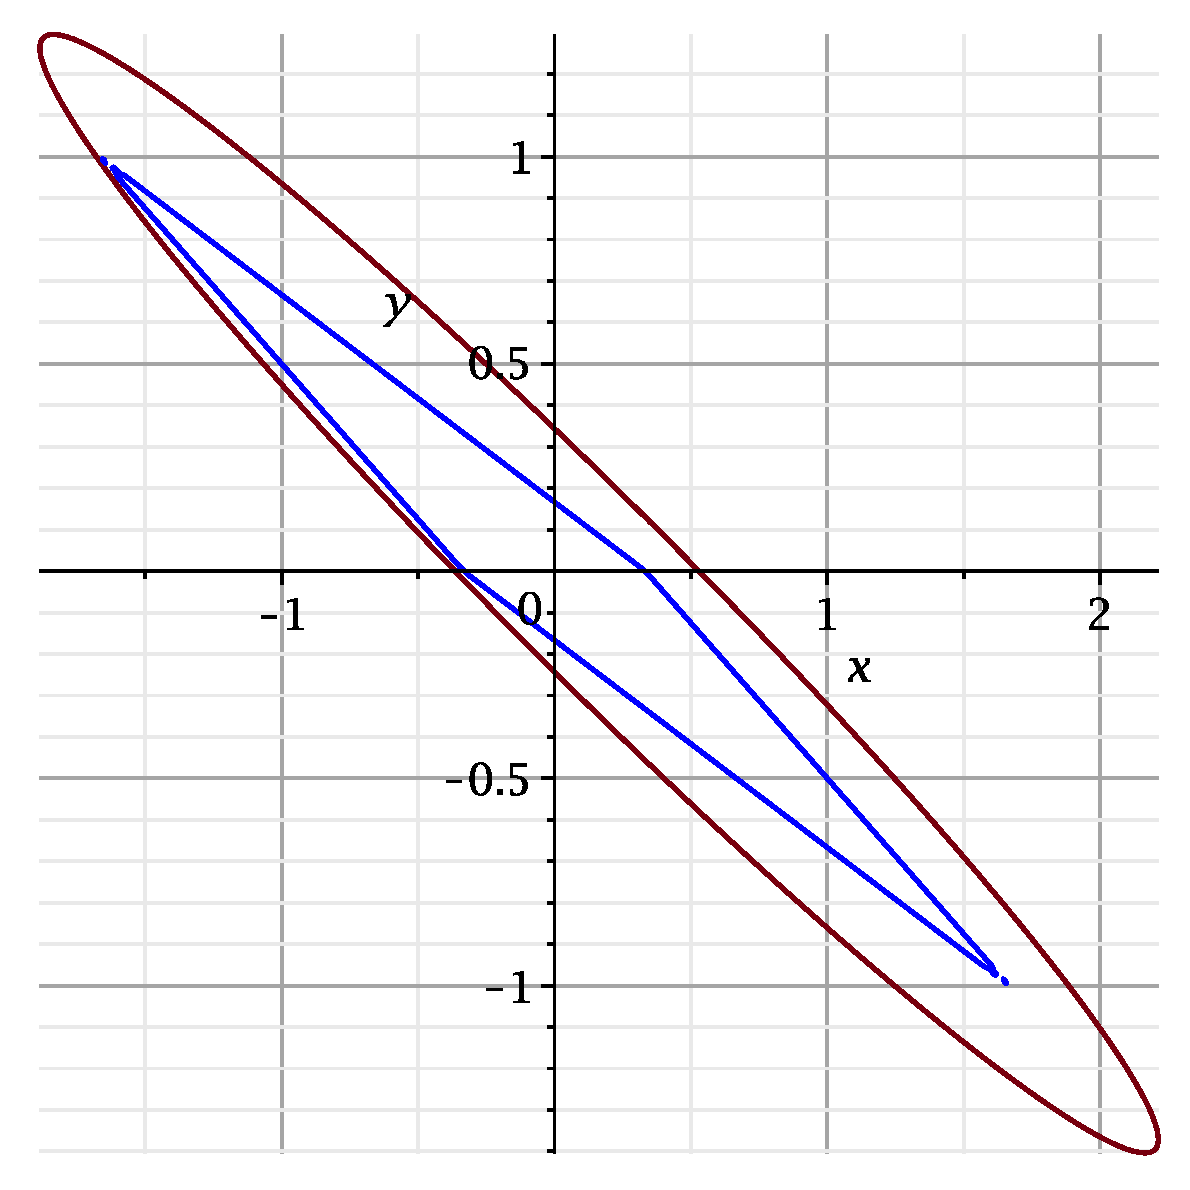
\includegraphics[width=.8\linewidth]{pictures/1_8.eps}
        \caption{E}
    \label{fig:sfig2}
    \end{subfigure}
\end{figure}

\end{frame}

\begin{frame}
$\|Av_{max}\| = 0.8195480889$  
    \begin{figure}
    \begin{subfigure}{.5\textwidth}
        \centering
        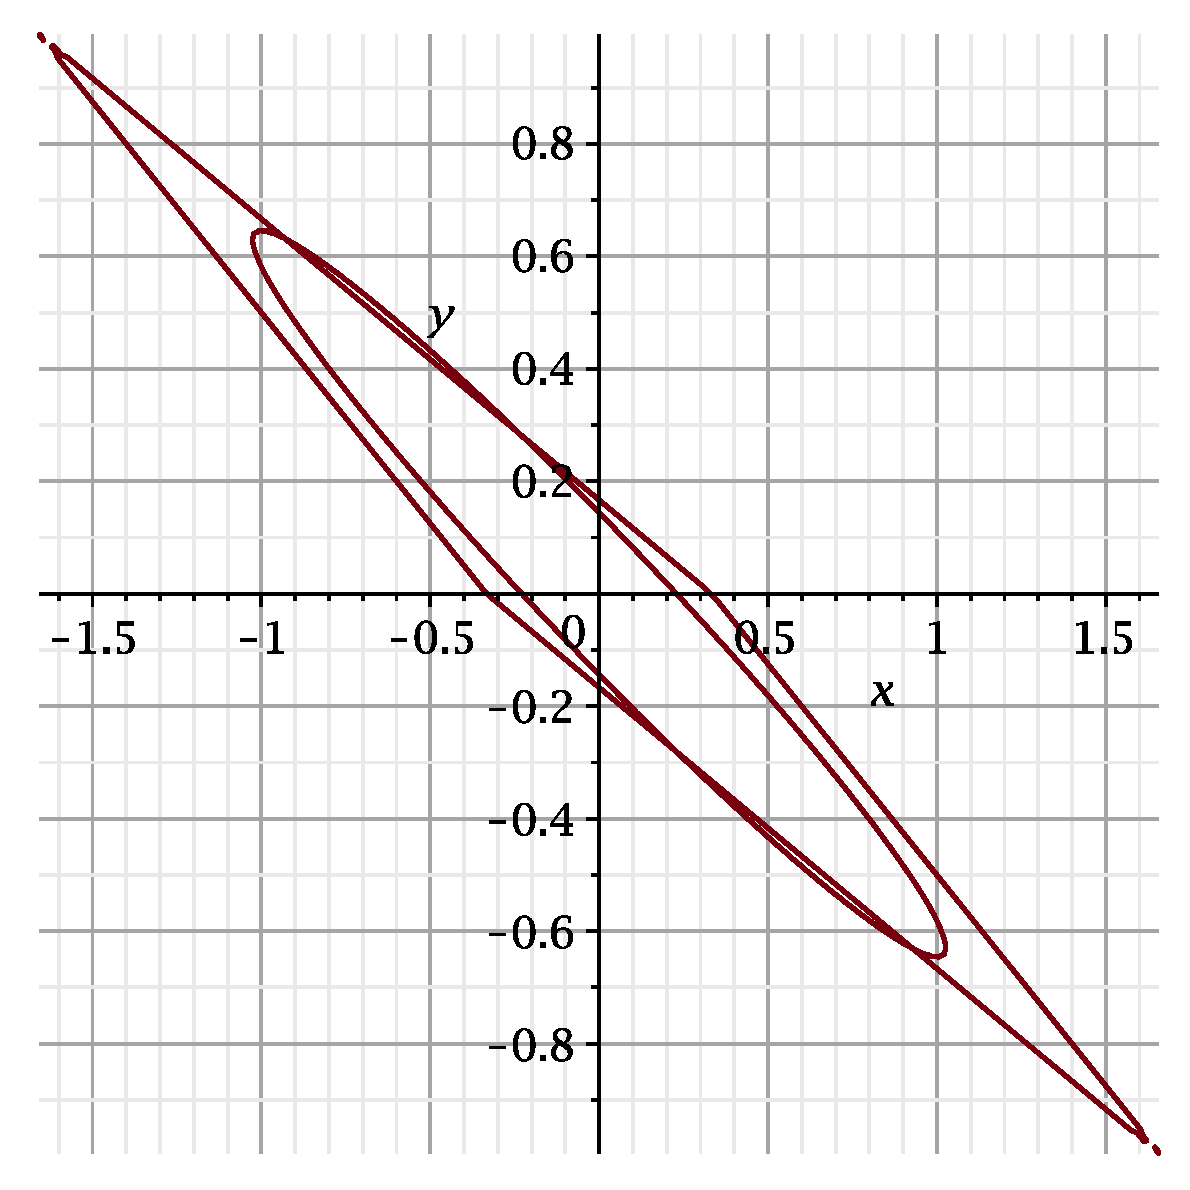
\includegraphics[width=.8\linewidth]{pictures/9.eps}
        \caption{$\displaystyle\frac{1}{d}(E-c)+c$}
    \label{fig:sfig1}
    \end{subfigure}%
    \begin{subfigure}{.5\textwidth}
        \centering
        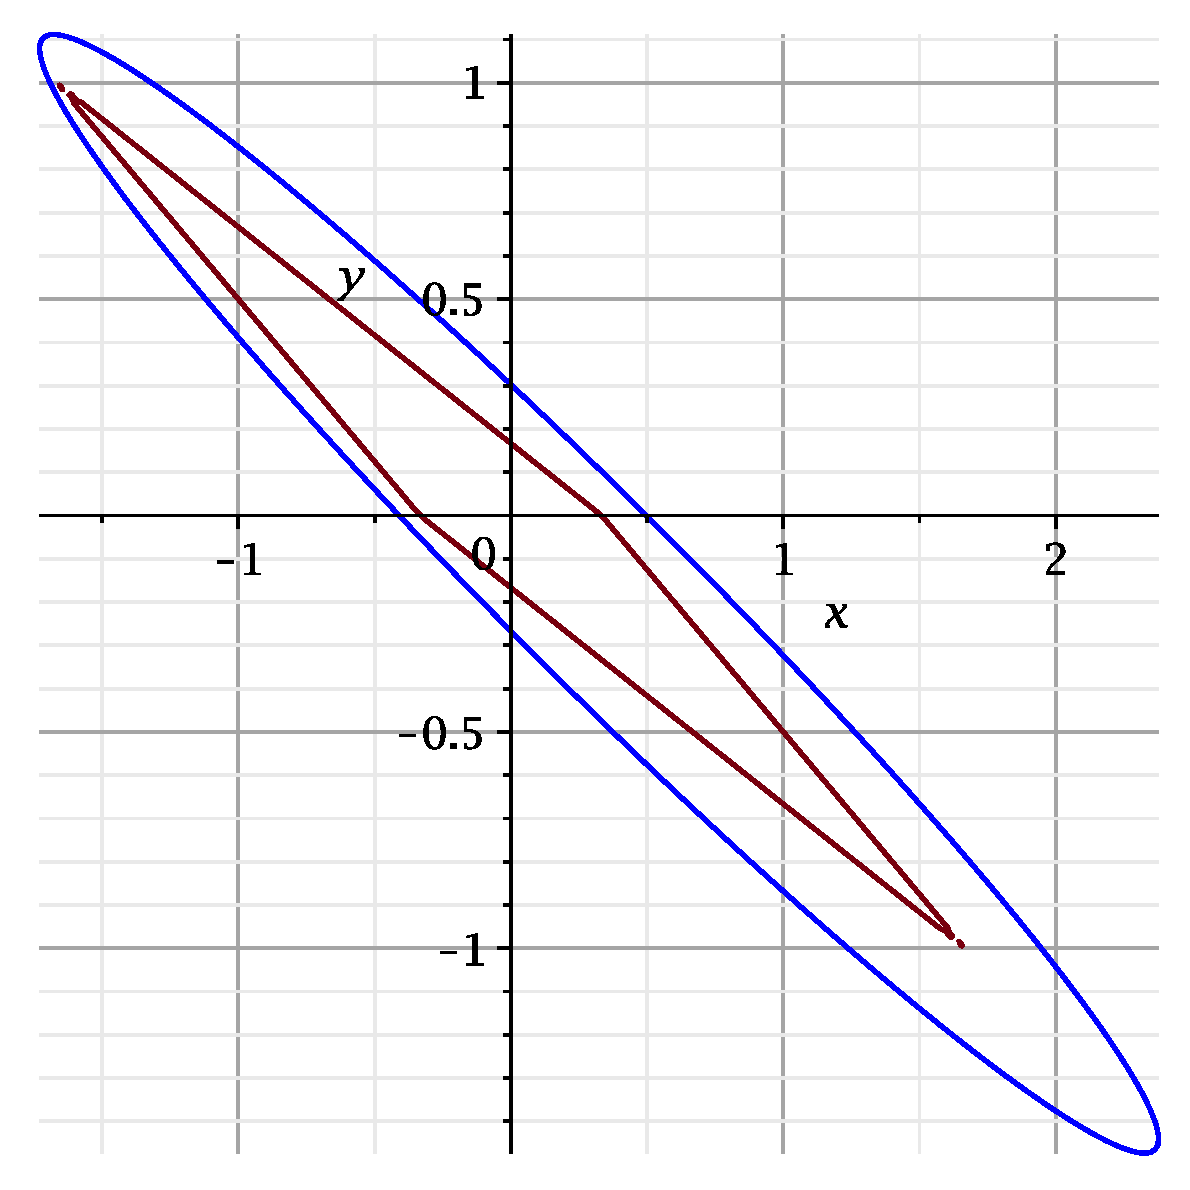
\includegraphics[width=.8\linewidth]{pictures/1_9.eps}
        \caption{E}
    \label{fig:sfig2}
    \end{subfigure}
\end{figure}

\end{frame}

\begin{frame}
$\|Av_{max}\| = 0.7980541166$  
    \begin{figure}
    \begin{subfigure}{.5\textwidth}
        \centering
        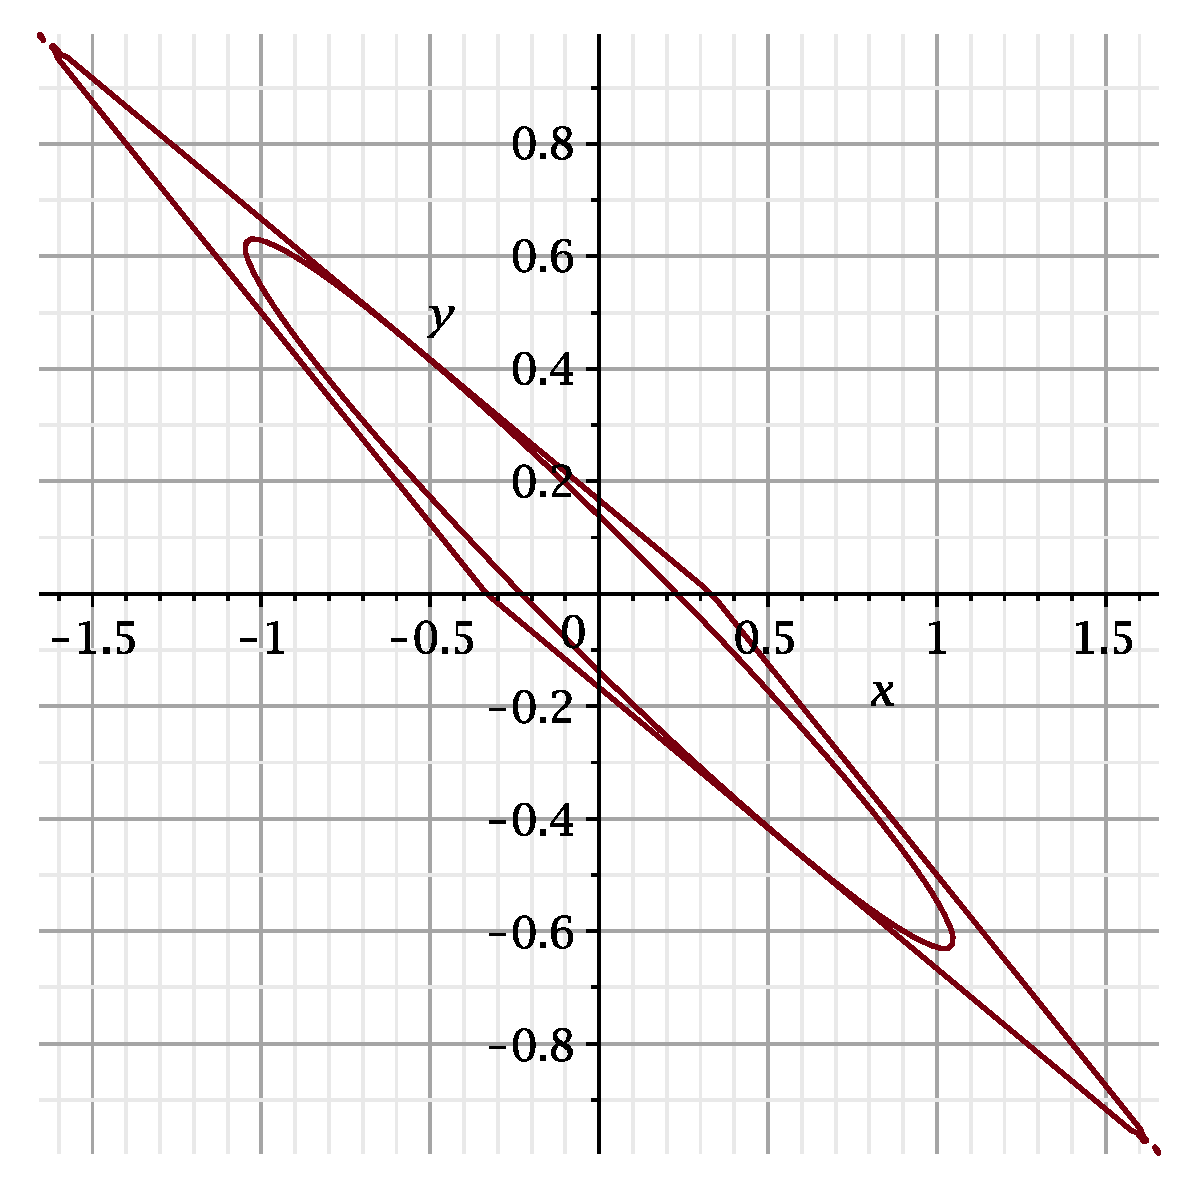
\includegraphics[width=.8\linewidth]{pictures/10.eps}
        \caption{$\displaystyle\frac{1}{d}(E-c)+c$}
    \label{fig:sfig1}
    \end{subfigure}%
    \begin{subfigure}{.5\textwidth}
        \centering
        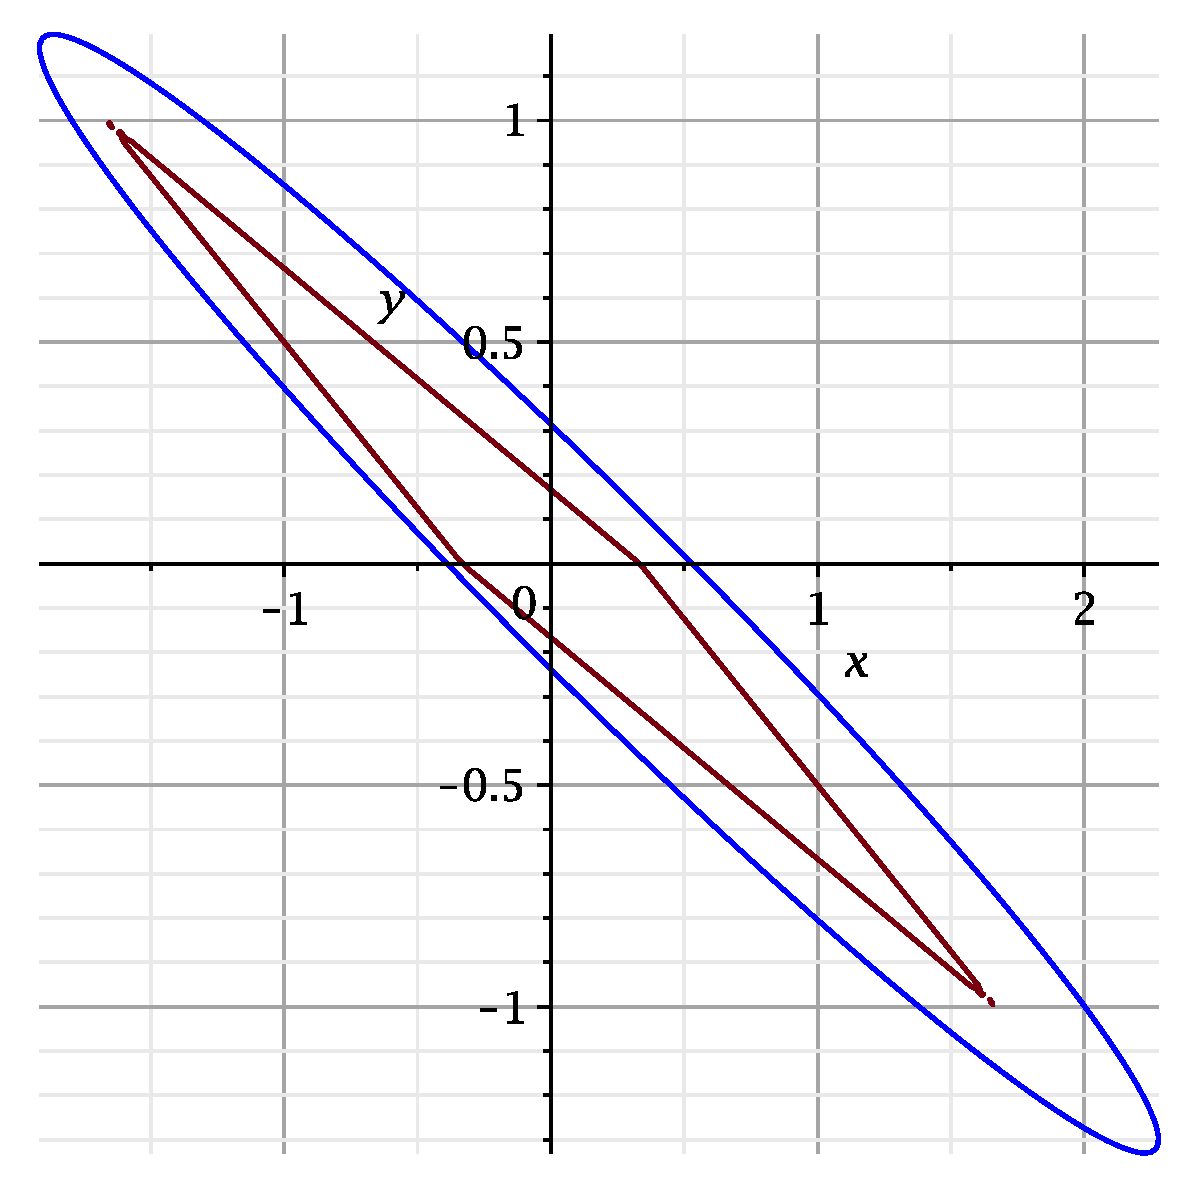
\includegraphics[width=.8\linewidth]{pictures/1_10.eps}
        \caption{E}
    \label{fig:sfig2}
    \end{subfigure}
\end{figure}

\end{frame}

\end{document} 
